%%%%%%%%%%%%%%%%%%%%%%%%%%%%%%%%%%%%%%%%%
% Beamer Presentation
% LaTeX Template
% Version 1.0 (10/11/12)
%
% This template has been downloaded from:
% http://www.LaTeXTemplates.com
%
% License:
% CC BY-NC-SA 3.0 (http://creativecommons.org/licenses/by-nc-sa/3.0/)
%
%%%%%%%%%%%%%%%%%%%%%%%%%%%%%%%%%%%%%%%%%

%----------------------------------------------------------------------------------------
%	PACKAGES AND THEMES
%----------------------------------------------------------------------------------------

\documentclass{beamer}

\mode<presentation> {

% The Beamer class comes with a number of default slide themes
% which change the colors and layouts of slides. Below this is a list
% of all the themes, uncomment each in turn to see what they look like.

%\usetheme{default}
%\usetheme{AnnArbor}
%\usetheme{Antibes}
%\usetheme{Bergen}
%\usetheme{Berkeley}
%\usetheme{Berlin}
%\usetheme{Boadilla}
%\usetheme{CambridgeUS}
%\usetheme{Copenhagen}
%\usetheme{Darmstadt}
%\usetheme{Dresden}
%\usetheme{Frankfurt}
%\usetheme{Goettingen}
%\usetheme{Hannover}
%\usetheme{Ilmenau}
%\usetheme{JuanLesPins}
%\usetheme{Luebeck}
%\usetheme{Madrid}
%\usetheme{Malmoe}
%\usetheme{Marburg}
%\usetheme{Montpellier}
%\usetheme{PaloAlto}
%\usetheme{Pittsburgh}
%\usetheme{Rochester}
%\usetheme{Singapore}
%\usetheme{Szeged}
\usetheme{Warsaw}

% As well as themes, the Beamer class has a number of color themes
% for any slide theme. Uncomment each of these in turn to see how it
% changes the colors of your current slide theme.

%\usecolortheme{albatross}
%\usecolortheme{beaver}
%\usecolortheme{beetle}
%\usecolortheme{crane}
%\usecolortheme{dolphin}
%\usecolortheme{dove}
%\usecolortheme{fly}
%\usecolortheme{lily}
%\usecolortheme{orchid}
%\usecolortheme{rose}
%\usecolortheme{seagull}
%\usecolortheme{seahorse}
%\usecolortheme{whale}
%\usecolortheme{wolverine}

%\setbeamertemplate{footline} % To remove the footer line in all slides uncomment this line
%\setbeamertemplate{footline}[page number] % To replace the footer line in all slides with a simple slide count uncomment this line

%\setbeamertemplate{navigation symbols}{} % To remove the navigation symbols from the bottom of all slides uncomment this line
}

\usepackage{graphicx} % Allows including images
\usepackage{booktabs} % Allows the use of \toprule, \midrule and \bottomrule in tables
\usepackage{pgf,pgfarrows,pgfnodes}
\usepackage{tikz}
\usepackage{algorithm,algorithmic}
\usepackage{tabularx}
\renewcommand{\algorithmicrequire}{\textbf{Input:}}
\renewcommand{\algorithmicensure}{\textbf{Output:}}
%\newtheorem{theorem}{Theorem}[section]
%\usepackage{algorithm2e}
%\usetikzlibrary{arrows,shapes,trees}
%----------------------------------------------------------------------------------------
%	TITLE PAGE
%----------------------------------------------------------------------------------------

\title[]{A Study On Causality} % The short title appears at the bottom of every slide, the full title is only on the title page

\author{Li ZHONG} % Your name
\institute[\'Ecole Polytechnique] % Your institution as it will appear on the bottom of every slide, may be shorthand to save space
{
Aldebaran Robotics \\ % Your institution for the title page
\medskip
\textit{lzhong@aldebaran-robotics.com} % Your email address
}
\date{\today} % Date, can be changed to a custom date

\begin{document}

\begin{frame}
\titlepage % Print the title page as the first slide
\end{frame}

\begin{frame}
\frametitle{Overview} % Table of contents slide, comment this block out to remove it
\tableofcontents % Throughout your presentation, if you choose to use \section{} and \subsection{} commands, these will automatically be printed on this slide as an overview of your presentation
\end{frame}

%----------------------------------------------------------------------------------------
%	PRESENTATION SLIDES
%----------------------------------------------------------------------------------------

%------------------------------------------------
%------------------------------------------------



\section{Introduction} % Sections can be created in order to organize your presentation into discrete blocks, all sections and subsections are automatically printed in the table of contents as an overview of the talk

% \begin{frame}
% \frametitle{Introduction}
% Causality is fundamental to many aspects of physics, economics, social science and
% human cognition. How can we know about causality structure?
% \\~\\

% Varies models including "Probabilistic Causation", "Causal Calculus", "Structure Learning"
% "Derivation Theories", "Manipulation Theories" etc.

% \end{frame}

% -----add new frames
\begin{frame}
Causality deals with the processing of three types of queries:

\begin{itemize}
\item predictions (e.g., would the pavement be slippery if
we find the sprinkler off?);
\item interventions (e.g., would the pavement be slippery if
we make sure that the sprinkler is off?); and
\item counterfactuals (e.g., would the pavement be slippery
had the sprinkler been off, given that the pavement
is in fact not slippery and the sprinkler is on?).
\end{itemize}

We shall see that these three types of queries represent a
hierarchy of three fundamentally different types of
problems, demanding knowledge with increasing levels of
detail.

\end{frame}



%------end adding

%------------------------------------------------
\section{Learning Causal Relations} % A subsection can be created just before a set of slides with a common theme to further break down your presentation into chunks

\subsection{Preliminaries}
\begin{frame}
\frametitle{Directed Acyclic Graph}
A causal structure of a set of variables V is a directed acylic graph (DAG) in which each node
corresponds direct element of V, and each link represents direct functional relationship
among the corresponding variables.
\\~\\

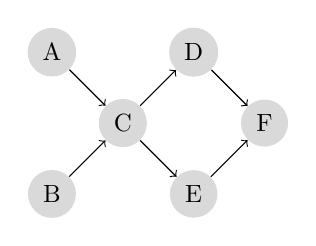
\begin{tikzpicture}[scale=.9, transform shape]
\tikzstyle{every node} = [circle, fill=gray!30]
\node (a) at (0, 2) {A};
\node (b) at (0, 0) {B};
\node (c) at (1, 1) {C};
\node (d) at (2, 2) {D};
\node (e) at (2, 0) {E};
\node (f) at (3, 1) {F};

%\draw [->] (a) -- (c)
\foreach \from/\to in {a/c, b/c, c/e,c/d,d/f,e/f}
\draw [->] (\from) -- (\to);
\end{tikzpicture}

A and B are causally independent;
C, D, E, and F are causally dependent on A and B;
A and B are direct causes C;
A and B are indirect causes D, E and F;
If C is prevented from changing with A and B, then A and B will no longer cause changes in D, E and F.
\end{frame}

%\subsection{Minimality}
\begin{frame}
\frametitle{Definitions}
\begin{itemize}
\item Structure Preference
\item Minimality
\item Consistency
\item Inferred Causation
\item Stability
\item Markov Parents
\end{itemize}
\end{frame}


\begin{frame}
\frametitle{Minimality}
A latent structure L is \textbf{minimal} with respect to a class $\mathbb{L}$
of latent structures if and only if there is no member of $\mathbb{L}$ that is
strictly preferred to L -- that is , if and ony if for every $L^{'} \in \mathbb{L}$
we have $L \equiv L^{'}$ whenever $L^{'} \succeq L$.
\end{frame}

\begin{frame}
\frametitle{Minimality}
\begin{figure}
\includegraphics[width=0.7\textwidth]{/home/lzhong/Pictures/Selection_001.png}
\caption{Examples}
\end{figure}
\end{frame}

% \begin{frame}
% \frametitle{Stability}
% The stability condition states that, as we vary the $\psi$
% parameters from to $\psi^'$, no independence in $P$ can be
% destroyed.
% \end{frame}

\subsection{Inductive Causation Algorithm}
\begin{frame}
\frametitle{IC algorithm}
\begin{itemize}
\item  Based on variable dependencies;
\item  Find all pairs of variables that are dependent of each other (applying standard statistical method on the database);
\item  Eliminate (as much as possible) indirect dependencies;
Determine directions of dependencies;
\end{itemize}
\end{frame}

\begin{frame}
\frametitle{IC algorithm}

\begin{algorithm}[H]
\begin{algorithmic}[1]
\REQUIRE{P -- a stable distribution on a set $V$ of variables}
\STATE each pair of variables $a$ and $b$ in $V$, search for a set $S_{ab}$ such that $a\perp b | S_{ab}$ holds in P – in other words, $a$ and $b$ should be independent in P, conditioned on $S_{ab}$ . 
\STATE construct an undirected graph G such that vertices $a$ and $b$ are connected with an edge if and only if no set $S_{ab}$ can be found.
\STATE for each pair of nonadjacent variables $a$ and $b$ with a common neighbor $c$, check if $c \in S_{ab}$.
\STATE if it is, then continue; else add arrowheads at $c$.
\ENSURE{A pattern H(P) compatible with P}
\end{algorithmic}
\caption{IC algorithm}
\label{alg:seq}
\end{algorithm}
\end{frame}

\begin{frame}
\frametitle{Orientation}
In the partially directed graph that results, orient as many of the undirected edges as possible subject to two conditions:
\begin{itemize}
\item  The orientation should not create a new v-structure;
\item  The orientation should not create a directed cycle;
\end{itemize}
\end{frame}

% \begin{frame}
% \frametitle{Orientation}
% In practice, we have 4 rules required to obtaining a maximally oriented pattern:
% \begin{itemize}
% \item  Orient $b - c$  into $b \to c$ whenever there is an arrow $a\to b$ such that $a$ and $c$ are non adjacent;
% \end{itemize}
% \\~\\

% \begin{tikzpicture}[scale=.9, transform shape]
% \tikzstyle{every node} = [circle, fill=gray!30]
% \node (b) at (0, 0) {b};
% \node (c) at (1, 0) {c};
% \draw  (b) -- (c);
% \end{tikzpicture}

% \begin{tikzpicture}[scale=.9, transform shape]
% \tikzstyle{every node} = [circle, fill=gray!30]
% \node (a) at (0, 0) {a};
% \node (b) at (1, 0) {b};
% \node (c) at (2, 0) {c};
% %\node (d) at (2, 2) {D};
% % \node (e) at (2, 0) {E};
% % \node (f) at (3, 1) {F};

% \draw [->] (a) -- (b);
% \draw  (b) -- (c);

% %\foreach \from/\to in {a/c, b/c, c/e,c/d,d/f,e/f}
% %\draw [->] (\from) -- (\to);
% \end{tikzpicture}

% % \item  Orient $a - b$  into $a\to b$ whenever there are two chains $a-c\to d$  and $c\to d\to b$ such that $c$ and $b$ are nonadjacent;

% %\end{itemize}
% \end{frame}

\begin{frame}
\frametitle{Orientation}
\begin{itemize}
\item  Orient $a - b$  into $a\to b$ whenever there is a chain $a\to c\to b$;

\end{itemize}
\\~\\

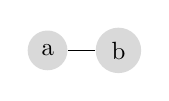
\begin{tikzpicture}[scale=.9, transform shape]
\tikzstyle{every node} = [circle, fill=gray!30]
\node (a) at (0, 0) {a};
\node (b) at (1, 0) {b};
\draw  (a) -- (b);
\end{tikzpicture}

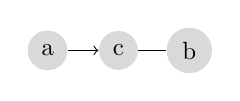
\begin{tikzpicture}[scale=.9, transform shape]
\tikzstyle{every node} = [circle, fill=gray!30]
\node (a) at (0, 0) {a};
\node (c) at (1, 0) {c};
\node (b) at (2, 0) {b};
%\node (d) at (2, 2) {D};
% \node (e) at (2, 0) {E};
% \node (f) at (3, 1) {F};

\draw [->] (a) -- (c);
\draw  (c) -- (b);

% %\foreach \from/\to in {a/c, b/c, c/e,c/d,d/f,e/f}
% %\draw [->] (\from) -- (\to);
\end{tikzpicture}

\end{frame}

\begin{frame}
\frametitle{Orientation}
\begin{itemize}
\item  Orient $a - b$  into $a\to b$ whenever there are two chains $a-c\to b$ and $a-d\to b$ such that $c$ and $d$ are nonadjacent;
\end{itemize}
\\~\\

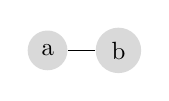
\begin{tikzpicture}[scale=.9, transform shape]
\tikzstyle{every node} = [circle, fill=gray!30]
\node (a) at (0, 0) {a};
\node (b) at (1, 0) {b};
\draw  (a) -- (b);
\end{tikzpicture}

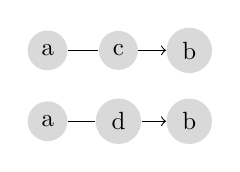
\begin{tikzpicture}[scale=.9, transform shape]
\tikzstyle{every node} = [circle, fill=gray!30]
\node (a) at (0, 0) {a};
\node (c) at (1, 0) {c};
\node (b) at (2, 0) {b};
\node (b1) at (2, -1) {b};
\node (a1) at (0, -1) {a};
\node (d) at (1, -1) {d};
% \node (e) at (2, 0) {E};
% \node (f) at (3, 1) {F};

\draw (a) -- (c);
\draw [->] (c) -- (b);
\draw (a1) -- (d);
\draw [->] (d) -- (b1);

%\foreach \from/\to in {a/c, b/c, c/e,c/d,d/f,e/f}
%\draw [->] (\from) -- (\to);
\end{tikzpicture}
\end{frame}

\begin{frame}
\frametitle{Orientation}
\begin{itemize}
\item  Orient $a - b$  into $a\to b$ whenever there are two chains $a-c\to d$ and $c\to d\to b$ such that $c$ and $b$ are nonadjacent;
\end{itemize}
\\~\\

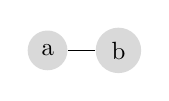
\begin{tikzpicture}[scale=.9, transform shape]
\tikzstyle{every node} = [circle, fill=gray!30]
\node (a) at (0, 0) {a};
\node (b) at (1, 0) {b};
\draw  (a) -- (b);
\end{tikzpicture}

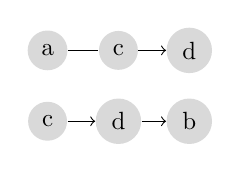
\begin{tikzpicture}[scale=.9, transform shape]
\tikzstyle{every node} = [circle, fill=gray!30]
\node (a) at (0, 1) {a};
\node (c1) at (1, 1) {c};
\node (b) at (2, 0) {b};
\node (d1) at (2, 1) {d};
\node (d2) at (1, 0) {d};
\node (c2) at (0, 0) {c};

% \node (e) at (2, 0) {E};
% \node (f) at (3, 1) {F};

\draw  (a) -- (c1);
\draw [->] (c1) -- (d1);
\draw [->] (c2) -- (d2);
\draw [->] (d2) -- (b);

% %\foreach \from/\to in {a/c, b/c, c/e,c/d,d/f,e/f}
% %\draw [->] (\from) -- (\to);
\end{tikzpicture}

\end{frame}

\section{Inferring Causal Relations}
\subsection{Causal Calculus}

\begin{frame}
\frametitle{classical example}

% \footnotesize Consider an experiment in which soil
% fumigants $(X)$ are used to increase oat crop yields $(Y)$ by
% controlling the eelworm population $(Z)$; the fumigants may
% also have direct effects (both beneficial and adverse) on
% yields besides the control of eelworms. 

\footnotesize A hypothetical data set from a study on the
relations among tar, cancer, and cigarette smoking is
presented in Table. Regardless of each of
these two groups (tar and no-tar), smokers show a muchhigher percentage of cancer than non-smokers.

% \footnotesize the quantities $Z_1$, $Z_2$, $Z_3$ represent the eelworm
% population before treatment, after treatment, and at the end
% of the season, respectively. The $Z_0$ term represents last
% year’s eelworm population. $B$ is the population of birds and other predators.

\footnotesize However, the tobacco industry
might argue that the table tells a different story – that
smoking actually decreases one’s risk of lung cancer. since the table shows that tar deposits have a protective effect in both groups.

\footnotesize To settle the dispute, we wish to calculate the probability
that a randomly selected person will develop cancer under
each of the following two actions: smoking (setting X = 1)
or not smoking (setting X = 0).

\begin{figure}
\includegraphics[width=0.8\textwidth]{/home/lzhong/Pictures/Selection_004.png}
%\caption{A causal diagram representing the effect of fumigants $(X)$ on
%yields $(Y)$}
\end{figure}



\end{frame}

\begin{frame}
\frametitle{Causal Calculus}
\small Causal calculus means mathematical machineary for performing the computational tasks
to inference intervention effects in a causal network, which is, more specifically, 
to calculate the $P(A|do(B))$.
\begin{theorem}
Let $PA_i$ denote the set of direct causes of variable $X_i$ and
let $Y$ be any set of variables disjoint of ${X_i PA_i}$ . The
effect of the intervention $do(x_i = \hat{x_i})$ on $Y$ is given by
$$
P(y|\hat{x_i}) = \sum_{pa_i} P(y|\hat{x_i},pa_i)P(pa_i)
$$
where $P(y|\hat{x_i}, pa_i)$ and $P(pa_i)$ represent preintervention
probabilities.
\end{theorem}

\end{frame}

\begin{frame}

Proof:
$$\\
P(x_1,...,x_n|\hat{x_i}) =\begin{cases} \frac{P(x_1,...,x_n)}{P(\hat{x_i}|pa_i)} &  x_i=\hat{x_i} \\ 0 &  x_i\neq \hat{x_i} \end{cases}

P(pa_i|\hat{x_i}) = \frac{P(pa_i,\hat{x_i})}{P(\hat{x_i})};

P(\overline{x_i}) = P( \overline{x_i}|pa_i);

P(x_1,...,x_n|\hat{x_i},pa_i) = \frac{P(x_1,...,x_n)}{P(\hat{x_i},pa_i)}

P(pa_i|\hat{x_i}) = P(pa_i);
$$\\


Thus:
$$
P(x_1,...,x_n|\hat{x_i}) =\begin{cases} P(x_1,...,x_n|\hat{x_i},pa_i)P(pa_i) &  x_i=\hat{x_i} \\ 0 &  x_i\neq \hat{x_i} \end{cases}\\
$$
% $$
% P(x_1,...,x_n|x_i^{'}) =\begin{cases} \prod_{j\neq i} P(x_j|pa_j) &  x_i=x_i^{'} \\ 0 &  x_i\neq x_i^{'} \end{cases}\\
% $$


%A key benefit of intervention is that it can distinguish between causal models
%that are difficult or impossible to discriminate by correlational data alone.

\end{frame}

\begin{frame}

\begin{columns}
\begin{column}{.48\textwidth}
%\color{red}\rule{\linewidth}{4pt}

\begin{definition}[Back-Door]
\scriptsize A set of variables $Z$ satisfies the back-door criterion
relative to an ordered pair of variables $(X_j , X_i)$ in a DAG
$G$ if:
\begin{itemize}
\item [i] no node in $Z$ is a descendant of $X_i$ ;
\item [ii] $Z$ blocks every path between $X_i$ and $X_j$ that
contains an arrow into $X_i$ .
\end{itemize}
\end{definition}

\begin{theorem}[Back-Door]
\scriptsize If a set of variables $Z$ satisfies the back-door criterion
relative to $(X, Y)$ , then the causal effect of $X$ on $Y$ is
$$
P(y|\hat{x}) = \sum_{z} P(y|x,z)P(z)
$$
\end{theorem}

\end{column}%
\hfill%
\begin{column}{.48\textwidth}
%\color{blue}\rule{\linewidth}{4pt}

\begin{definition}[Front-Door]
\scriptsize A set of variables $Z$ satisfies the front-door criterion
relative to an ordered pair of variables $(X_j , X_i)$ in a DAG
$G$ if:
\begin{itemize}
\item [i] $Z$ intercepts every directed path from $X_j$ to $X_i$;
\item [ii] no unbloked back-door path from $X_j$ to $Z$ ;
\item [iii] all back-door paths from $Z$ to $X_i$ are blocked by $X_j$
\end{itemize}
\end{definition}

\begin{theorem}[Front-Door]
\scriptsize If a set of variables $Z$ satisfies the front-door criterion
relative to $(X, Y)$ , and if $P(x,z)>0$ then the causal effect of $X$ on $Y$ is
$$
P(y|\hat{x}) = \sum_{z} P(z|x)\sum_{x^{'}}P(y|z,x^{'})P(x^{'})
$$
\end{theorem}

\end{column}%
\end{columns}


\end{frame}


\begin{frame}
\frametitle{Example}

\begin{figure}
\includegraphics[width=0.8\textwidth]{/home/lzhong/Pictures/Selection_004.png}
%\caption{A causal diagram representing the effect of fumigants $(X)$ on
%yields $(Y)$}
\end{figure}


\begin{figure}
\includegraphics[width=0.8\textwidth]{/home/lzhong/Pictures/Selection_005.png}
%\caption{A causal diagram representing the effect of fumigants $(X)$ on
%yields $(Y)$}
\end{figure}

\end{frame}
% \frametitle{Causal Calculus}
%------------------------------------------------
%\section{Approaches for computation}

\begin{frame}
\frametitle{Causal Calculus}
Let $G$ be a directed acyclic graph, let $P$ stand for the associated probability distribution. $X,Y,Z,W$ denote disjoint subsets of variables. $\underline{x}$ denotes intervetion on $x$. 

Further, we denote the following subgraphs of $G$:
\begin{itemize}
\item [-] $G_{\overline{X}}$ : remove arrows pointing to $X$
\item [-] $G_{\underline{X}}$ : remove arrows emanating from $X$
\item [-] $G_{\overline{X}\underline{Z}}$ : remove ears of $X$ and legs of $Z$
\item [-] $Z(W)$: the set of $Z$-nodes that are not ancestors of any $W$-nodes
\end{itemize}

\end{frame}

\begin{frame}
\frametitle{Causal Calculus}
\begin{block}{Rule 1: Insertion/deletion of observations}
\begin{equation}
P(y|\hat{x},z,w) = P(y|\hat{x},w), if (Y \perp Z |X,W)_{G_{\overline{X}}}
\end{equation}
\end{block}

\begin{block}{Rule 2: Action/observation exchange}
\begin{equation}
P(y|\hat{x},\hat{z},w) = P(y|\hat{x},z,w), if (Y \perp Z |X,W)_{G_{\overline{X}\underline{Z}}}
\end{equation}
\end{block}

\begin{block}{Rule 3: Insertion/deletion of actions}
\begin{equation}
P(y|\hat{x},z,w) = P(y|\hat{x},w), if (Y \perp Z |X,W)_{G_{\overline{X},\overline{Z(W)}}}
\end{equation}
\end{block}

\end{frame}


%%----------------------------------------------------------------------------

\subsection{Actions, Plans}

\begin{frame}
\frametitle{Actions}
$X$ is made to respond in a specified way to some set $Z$ of other
variables – say, through a functional relationship $x = g(z)$.\\
Let $P(y | do(X = g(z)))$ stand for the distribution (of $Y$)
prevailing under the policy $do(X = g(z))$. \\
To compute $P(y | do(X = g(z)))$, we condition on $Z$ and write
$$
\begin{array}{lcl}
P(y | do(X = g(z))) &=&  \sum_z P(y | do(X = g(z)), z) P(z| do(X = g(z)))\\
&=& \sum_z P(y |\hat{x},x)_{X = g(z)} P(z) \\
&=& \mathbb{E}_z[P(y | \hat{x},z)_{do(X = g(z))}] 
\end{array}
$$
\end{frame}

\begin{frame}
\frametitle{Plans}
\begin{definition}
A control problem consists of a directed acyclic graph
(DAG) $G$ with vertex set $V$, partitioned into four disjoint
sets V = {X, Z, U, Y}, where
\begin{itemize}
\item $X$ = the set of control variables (exposures,
interventions, treatments, etc.);
\item $Z$ = the set of observed variables, often called
covariates;
\item $U$ = the set of unobserved (latent) variables; and
\item $Y$ = an outcome variable
\end{itemize}
\end{definition}
\end{frame}

\begin{frame}
\frametitle{Plans}
We let the control variables be ordered $X = X_1 , X _2 ,...,
X_n$ such that every $X_k$ is a nondescendant of $X_{k + j} (j > 0)$ in
$G$, and we let the outcome $Y$ be a descendant of $X_n$ . Let $N_k$
stand for the set of observed nodes that are
nondescendants of any element in the set {$X_k , X_{k + 1}, ...,
X_n $}. A \emph{plan} $(\hat{x_1},...,\hat{x_n})$ is an ordered sequence
of value assignments to the control variables. 
A conditional plan $(\hat{g_1(z_1)},...,\hat{g_n(z_n)})$ is an ordered sequence
where each $g_k$ is a function from a
set $Z_k$ to $X_k$ and where $\hat{g_k(z_k)}$
stands for the statement “set
$X_k$ to $g_k(z_k)$ whenever $Z_k$ attains the value $z_k$ .” The
support $Z_k$ of each $g_k(z_k )$ function must not contain any
variables that are descendants of $X_k$ in $G$.


Our problem is to evaluate an unconditional plan  by
computing $P(y|\hat{x_1},...,\hat{x_n})$
which represents the impact of
the plan $(\hat{x_1},...,\hat{x_n})$
on the outcome variable $Y$.
\end{frame}


\begin{frame}
\frametitle{Plans}
Solution:\\
$$
P(y|\hat{x_1},...,\hat{x_n}) =\\
 \sum_{z_1,...,z_n} P(y|z_1,...,z_n,x_1,...,x_n)\prod_{k=1}^n P(y|z_1,...,z_{k-1},x_1,...,x_{k-1})
$$
\end{frame}

\subsection{Simpon's Paradox}

\begin{frame}
\frametitle{Simpon's Paradox}

\begin{table}
\begin{tabular}{l l l}
\toprule
 & Treatment A  & Treatment B \\
\midrule
Small Stones & Group 1 & Group 2 \\
& 93\% (81/87) & 87\% (234/270) \\
Large Stones & Group 3 & Group 4 \\
& 73\% (192/263) & 69\% (55/80) \\
\\
Both & 78\% (273/350) &	83\% (289/350) \\
\bottomrule
\end{tabular}
\caption{Simpon's paradox, 1951-1994}
\end{table}

\end{frame}

%------------------------------------------------

\begin{frame}
\frametitle{Simpon's Reversal}
\begin{columns}[c] % The "c" option specifies centered vertical alignment while the "t" option is used for top vertical alignment

\column{.45\textwidth} % Left column and width
\textbf{Reversal}
\begin{enumerate}
\item Group 1 $>$ Group 2
\item Group 3 $>$ Group 4
\item Group 1 "+" Group 3 $<$ Group 2 "+" Group 4
\end{enumerate}

\column{.5\textwidth} % Right column and width
Even though Treatment A beats Treatment B in both separate experiments, however, the advantages of higher 
rate can easily be canceled with certain different proportions.

\end{columns}
\end{frame}

%------------------------------------------------
%\section{Second Section}
%------------------------------------------------


%------------------------------------------------

\begin{frame}
\frametitle{The Sure Thing Principle}
However, causal calculus prohibits reversal. In fact, we have following theorem:
\begin{theorem}
An action C that increases the probability of an event E in each subpopulation must also
increase the probability of E in the population as a whole
provided that the action does not change the distribution of the subpopulations.
\end{theorem}
\end{frame}

%------------------------------------------------

% \subsection{Temporal Order}

% \begin{frame} % Need to use the fragile option when verbatim is used in the slide
% \frametitle{Temporal Order}
% \begin{itemize}
% \item Temporal order of events provides a basic cue to causal structure
% \item Causes occur before their effects
% \item But temporal order is a fallible cue
% \end{itemize}
% \end{frame}

% %------------------------------------------------

% \begin{frame}
% \frametitle{Temporal Order}
% \begin{itemize}
% \item Order alone does not identify unique model
% 	\begin{itemize}
% 		\item [–] B can regularly follow A, but both result from common cause C
% 	\end{itemize}
% \item Order of experiences may not reflect order of occurrence
% 	\begin{itemize}
% 		\item [–] We often infer temporal order of events from the order in which we receive information about them
% 		\item [–] But sometimes we learn about an effect before we learn about the cause (e.g., find out about symptoms before disease)
% 	\end{itemize}
% \item But order can guide learning
% 	\begin{itemize}
% 		\item [–] Subjects use temporal order to construct initial model
% 		\item [–] Consistent data confirms this model – Add links to handle inconsistent data
% 	\end{itemize}
% \end{itemize}
% \end{frame}



\subsection{Counterfactual Analysis}
\begin{frame}
\frametitle{Counterfactuals}
What is conterfactual analysis?
\\~\\
$Y_x(u) = y$: $Y$ would be $y$, had $X$ been $x$ (in state $U=u$)
\end{frame}

\begin{frame}
\frametitle{Counterfactuals}
Conversion from graph to counterfactuals:
\begin{itemize}
\item Rule 1 (exclusion restrictions):\\
		for every variable $Y$ having parents $PA_Y$ and for every set of variables $Z \in V$
		disjoint of $PA_Y$, we have:
		$Y_{pa_Y}(u) = Y_{pa_Yz}(u)$
\item Rule 2 (independence restrictions):\\
		if $Z_1,...,Z_k$ is any set of nodes in $V$ not connected to $Y$ via paths containing
		only $U$ variables, we have :
		$Y_{pa_Y} \perp \{Z_{1_{pa_Y}},...,Z_{k_{pa_Y}}\}$\\
\end{itemize}
\end{frame}

\begin{frame}
\frametitle{Counterfactuals}
Given a casual graph $M = <V,U,\{f_i\},P(u) >$, query:\\
$P(Y_x = y|Z=z)$, $Z$ may be affected by $x$
\\~\\
Steps:\\ 
\begin{itemize}
\item Update $P(u)$ by $Z=z, P(u) \to P(u|x)$
\item Form the conditional model $M^z = <V,U,\{f_i\},P(u|z) >$
\item Form the submodel $M^z = <V,U,F_x,P(u|z) >$
\item Compute: $P(Y_x = y|Z=z) = P_{M_x^z}(Y=y)$
\end{itemize}
\end{frame}


\begin{frame}
\frametitle{Counterfactuals}
\begin{figure}
\includegraphics[width=0.5\textwidth]{/home/lzhong/Pictures/Selection_002.png}
\caption{Examples}
\end{figure}
\end{frame}

%------------------------------------------------
\section{Computational Models of Learning}

\begin{frame} % Need to use the fragile option when verbatim is used in the slide
\frametitle{Computational models}
Two main approaches:\\
Bayesian:
\begin{itemize}
\item [–] Assign priors across all possible models
\item [–] Compute posteriors given data by updating via Bayes’ rule
\end{itemize}
Constraint-based:
\begin{itemize}
\item [-]Compute all dependencies and conditional dependencies in data
\item [–] Return graph structures that are consistent with these dependencies
\end{itemize}
\end{frame}


\begin{frame}
\frametitle{more examples}
Suppose there is a probability that the air of any day in a month is polluted
and you have a friend who regularly visit you and smoke in your house. The robot wants to know whether it is useful to use air clearner.


\begin{table}[htb]
\begin{tabularx}{\textwidth}{l l l l l}
\toprule
 & force AC off & force AC on & AC off & AC on\\
\midrule
Air quality is bad & 10 & 1 & 3 & 3 \\
Air quality is good & 20 & 29 & 12 & 12 \\
Days & 30 & 30 & 15 & 15 \\
\bottomrule
\end{tabularx}
%\caption{Simpon's paradox, 1951-1994}
\end{table}



\end{frame}

\begin{frame}
\frametitle{Discussions}
Causality deals with high-level events, while sensormotors face low-level information flows;\\
Causality deals with probabilities\& possibilities, while sensormotors deal with physical laws;\\
Causality is suitable for posterior analysis/explanation
\end{frame}

%------------------------------------------------

% \begin{frame}
% \frametitle{References}
% \footnotesize{
% \begin{thebibliography}{99} % Beamer does not support BibTeX so references must be inserted manually as below
% \bibitem[Smith, 2012]{p1} John Smith (2012)
% \newblock Title of the publication
% \newblock \emph{Journal Name} 12(3), 45 -- 678.
% \end{thebibliography}
% }
% \end{frame}

%------------------------------------------------

\begin{frame}
\Huge{\centerline{Thank you!}}
\end{frame}

%----------------------------------------------------------------------------------------

\end{document} 
